\documentclass[12pt, a4paper]{article}

\usepackage[hmargin=2.5cm, vmargin=2cm]{geometry}
\usepackage{amsthm, amssymb, mathtools, yhmath, graphicx}
\usepackage{fontspec, type1cm, titlesec, titling, fancyhdr, tabularx}
\usepackage{caption}
\usepackage{color}
\usepackage{hhline}
\usepackage{unicode-math}
\usepackage{nicefrac}
\usepackage[abbreviations]{siunitx}
\usepackage{comment}
\usepackage{float}
\usepackage{subcaption}

\usepackage[CheckSingle, CJKmath]{xeCJK}
\usepackage{CJKulem}
\usepackage{enumitem}
\usepackage[usenames, dvipsnames]{xcolor}
\usepackage{colortbl}
\usepackage{circuitikz}
%\setCJKmainfont[BoldFont=cwTex Q Hei]{cwTex Q Ming}
%\setCJKsansfont[BoldFont=cwTex Q Hei]{cwTex Q Ming}
%\setCJKmonofont[BoldFont=cwTex Q Hei]{cwTex Q Ming}
\setCJKmainfont[BoldFont=cwTeX Q Hei]{cwTeX Q Ming}

\def\normalsize{\fontsize{12}{18}\selectfont}
\def\large{\fontsize{14}{21}\selectfont}
\def\Large{\fontsize{16}{24}\selectfont}
\def\LARGE{\fontsize{18}{27}\selectfont}
\def\Huge{\fontsize{20}{30}\selectfont}

\titleformat{\section}{\bf\Large}{\arabic{section}}{24pt}{}
\titleformat{\subsection}{\large}{\arabic{subsection}.}{12pt}{}
\titlespacing*{\subsection}{0pt}{0pt}{1.5ex}

\parindent=24pt

\DeclarePairedDelimiter{\abs}{\lvert}{\rvert}
\DeclarePairedDelimiter{\norm}{\lVert}{\rVert}
\DeclarePairedDelimiter{\inpd}{\langle}{\rangle}
\DeclarePairedDelimiter{\ceil}{\lceil}{\rceil}
\DeclarePairedDelimiter{\floor}{\lfloor}{\rfloor}

\newcommand{\unit}[1]{\:(\text{#1})}
\newcommand{\img}{\mathsf{i}}
\newcommand{\ex}{\mathsf{e}}
\newcommand{\dD}{\mathrm{d}}
\newcommand{\dI}{\,\mathrm{d}}
\newcommand{\cpar}{\mathbin{\|}}
\DeclareSIUnit \uF {\micro \farad}
\DeclareSIUnit \mH {\milli \henry}

\title{ \bf {\huge 電子電路實驗9:二次線路的頻率響應}\\ 實驗預報}
\author{B02901178 江誠敏}
%\date{2014/09/21}

\begin{document}

\maketitle

\section{實驗目的}
在一個二次線路中,輸出不同頻率的正弦波會造成輸出波振幅及相位的改變。以頻率為 X 軸、 振幅為 Y 軸所繪出的圖即為頻率響應圖。本實驗即為求線性非時變二次電路(Linear Time-Invariant Second-Order Circuit)的頻率響應(Frequency Response)。


\section{實驗步驟}
\begin{enumerate}[itemsep=0pt]
  \item 以 LCR 計量測電容與電感的值。
  \item 將電路連接成如圖 9.1(a),其中 R = 2kΩ。
  \item 令 $v_i$ 為峰對峰值 1V 的弦波(1V 是信號產生器已接上電路的值),頻率依照每個數量級
  (decade)1, 2, 5 的順序由 200Hz 變化至 200kHz,記錄 $v_o$ 的峰對峰值。
  \item 令 $v_i$為峰對峰值 1V 的弦波(1V 是信號產生器已接上電路的值),頻率由 5kHz 線性變化至
  30kHz,記錄 $v_o$ 的峰對峰值。
  \item 將圖 9.1(a)改為 R = 510Ω ,重複步驟 3 與步驟 4。
  \item 將電路連接成如圖 9.1(b),其中 R = 2kΩ。
  \item 令 $v_i$ 為峰對峰值 1V 的弦波(1V 是信號產生器已接上電路的值),頻率依照每個數量級
  (decade)1, 2, 5 的順序由 200Hz 變化至 200kHz,記錄 $v_o$ 的峰對峰值。
  \item 令 $v_i$為峰對峰值 1V 的弦波(1V 是信號產生器已接上電路的值),頻率由 5kHz 線性變化至
  30kHz,記錄 $v_o$ 的峰對峰值。
  \item 將圖 9.1(a)改為 R = 510Ω ,重複步驟 7 與步驟 8。
  \item 將電路連接成如圖 9.1(c),其中 R =1kΩ 。
  \item 令 $v_i$ 為峰對峰值 1V 的弦波(1V 是信號產生器已接上電路的值),頻率依照每個數量級
  (decade)1, 2, 5 的順序由 200Hz 變化至 200kHz,記錄 $v_o$ 的峰對峰值。
  \item 令 $v_i$為峰對峰值 1V 的弦波(1V 是信號產生器已接上電路的值),頻率由 5kHz 線性變化至
  30kHz,記錄 $v_o$ 的峰對峰值。
  \item 將圖 9.1(c)改為 R = 2kΩ,重複步驟 11 與步驟 12。
  \item 將圖 9.1(c)改為 R = 510Ω ,重複步驟 11 與步驟 12。
\end{enumerate}


\section{預報問題}

\begin{enumerate}[itemsep=20pt, topsep=10pt]
  \item {\large\bf 請推導圖 9.1 的三個電路的轉換函數。} \\[10pt]
    以下令$s = \img \omega$。
    \begin{enumerate}[label=(\alph*)]
      \item \\
        We have
        \[
          (R \cpar Z_C) = \frac{R (1/(sC))}{R + (1/(sC))} = \frac{R}{1+sRC}
        \]
        So
        \begin{align*}
        V_o &= \frac{R \cpar Z_C}{Z_L + (R \cpar Z_C)} \\
            &= \frac{R/(1+sRC)}{sL + (R/(1+sRC))} \\
            &= \frac{R}{R + sL + s^2 LRC} 
        \end{align*}
        notice that
        \[
          \frac{R}{R + sL + s^2 LRC} \ll 1 ,\quad \text{if } s \gg 1
        \]
      \item \\
        We have
        \[
          (R \cpar Z_L) = \frac{R (sL)}{R + sL} = \frac{sRL}{R+sL}
        \]
        So
        \begin{align*}
        V_o &= \frac{R \cpar Z_L}{Z_C + (R \cpar Z_L)} \\
            &= \frac{(sRL)/(R+sL)}{(1/sC) + (sRL/(R+sL))} \\
            &= \frac{s^2LRC}{R + sL + s^2 LRC} 
        \end{align*}
        notice that
        \[
          \frac{s^2LRC}{R + sL + s^2 LRC} \ll 1 ,\quad \text{if } s \ll 1
        \]
      \item \\
        We have
        \[
          (Z_C \cpar Z_L) = \frac{(1/sC) (sL)}{(1/sC)+sL} = \frac{sL}{1+s^2LC}
        \]
        So
        \begin{align*}
        V_o &= \frac{Z_C \cpar Z_L}{R + (Z_C \cpar Z_L)} \\
            &= \frac{(sL)/(1+s^2LC)}{R + (sL)/(1+s^2LC)} \\
            &= \frac{sL}{R + sL + s^2 LRC} 
        \end{align*}
        notice that
        \begin{alignat*}{4}
          \frac{sL}{R + sL + s^2 LRC} &\sim O(s) \quad && \text{as} \quad && s \rightarrow 0 \\
          \frac{sL}{R + sL + s^2 LRC} &\sim O\left(\frac{1}{s}\right) \quad && \text{as} \quad && s \rightarrow \infty
        \end{alignat*}
        so
        \[
          \frac{sL}{R + sL + s^2 LRC} \ll 1 ,\quad \text{if } s \ll 1 \text{ or } s \gg 1
        \]

    \end{enumerate}
  \item {\large\bf 請用 PSpice 或其他電路模擬軟體,模擬圖 9.1 的電路,並設定C = 0.01μF, L =10mH , R = 510Ω /1kΩ / 2kΩ,利用交流分析的功能繪出頻率響應圖。} 
    \begin{enumerate}[label=(\alph*)]
      \item 低通電路  \begin{figure}[H]
        \centering
        \begin{subfigure}[b]{0.45\textwidth}
          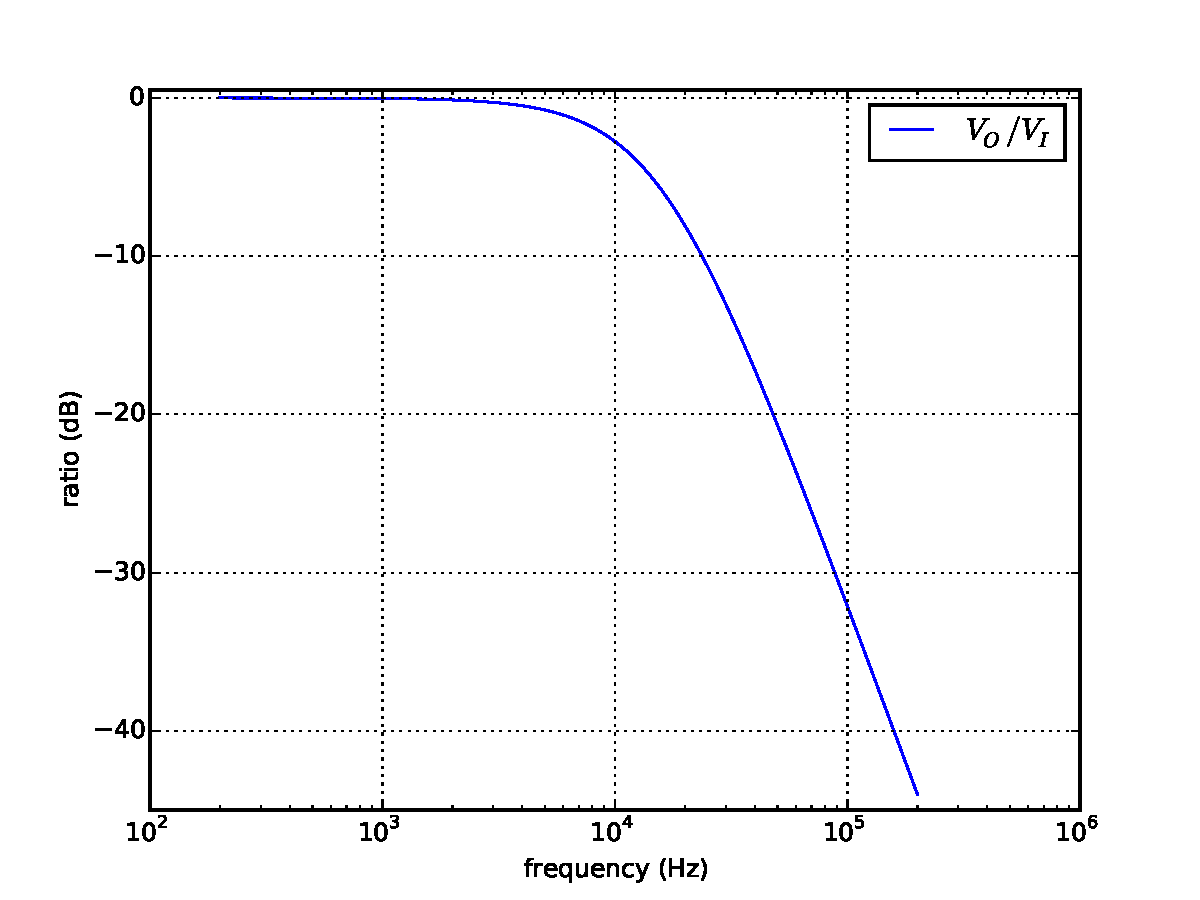
\includegraphics[width=1\textwidth]{circuit/p11.pdf}
          \caption{$\SI{510}\ohm$}
        \end{subfigure}
        \begin{subfigure}[b]{0.45\textwidth}
          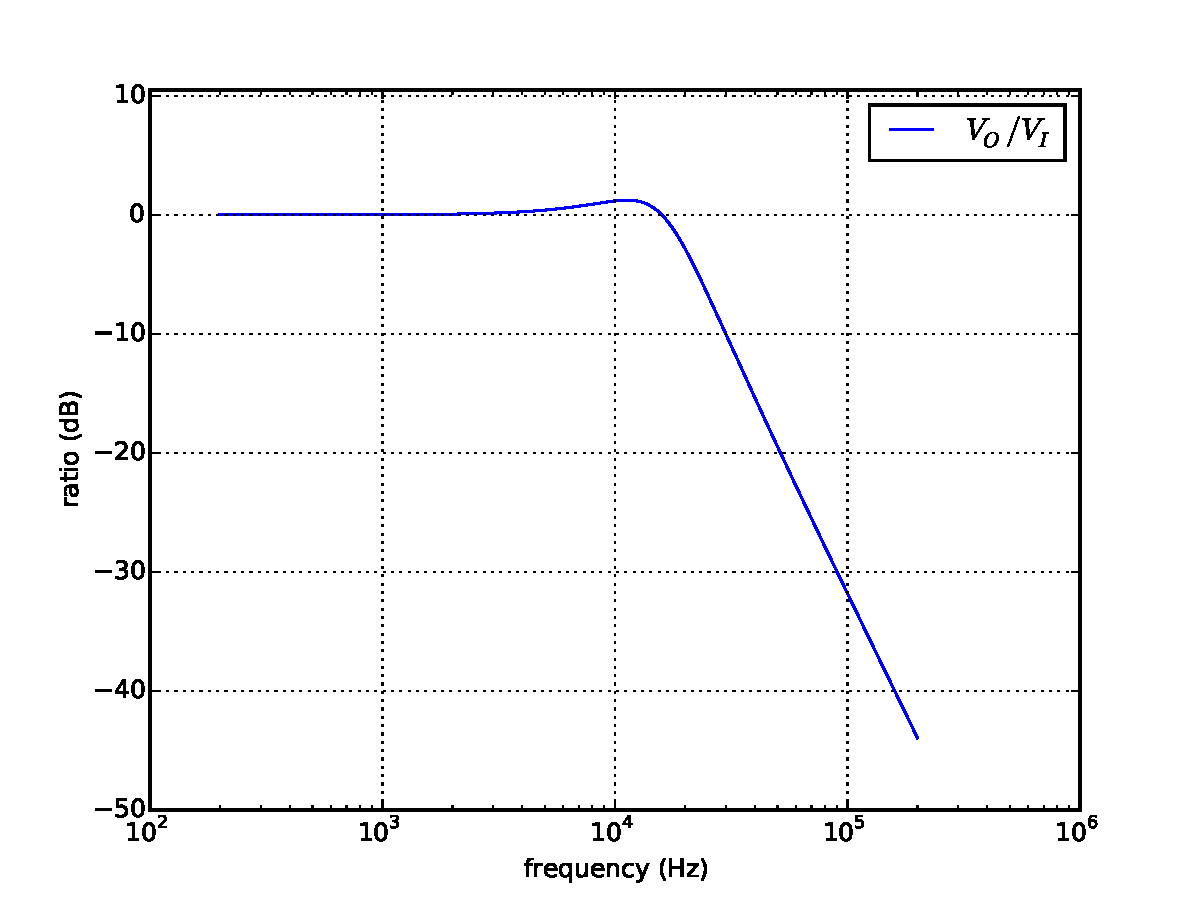
\includegraphics[width=1\textwidth]{circuit/p12.pdf}
          \caption{$\SI{1}\kohm$}
        \end{subfigure}
        \begin{subfigure}[b]{0.45\textwidth}
          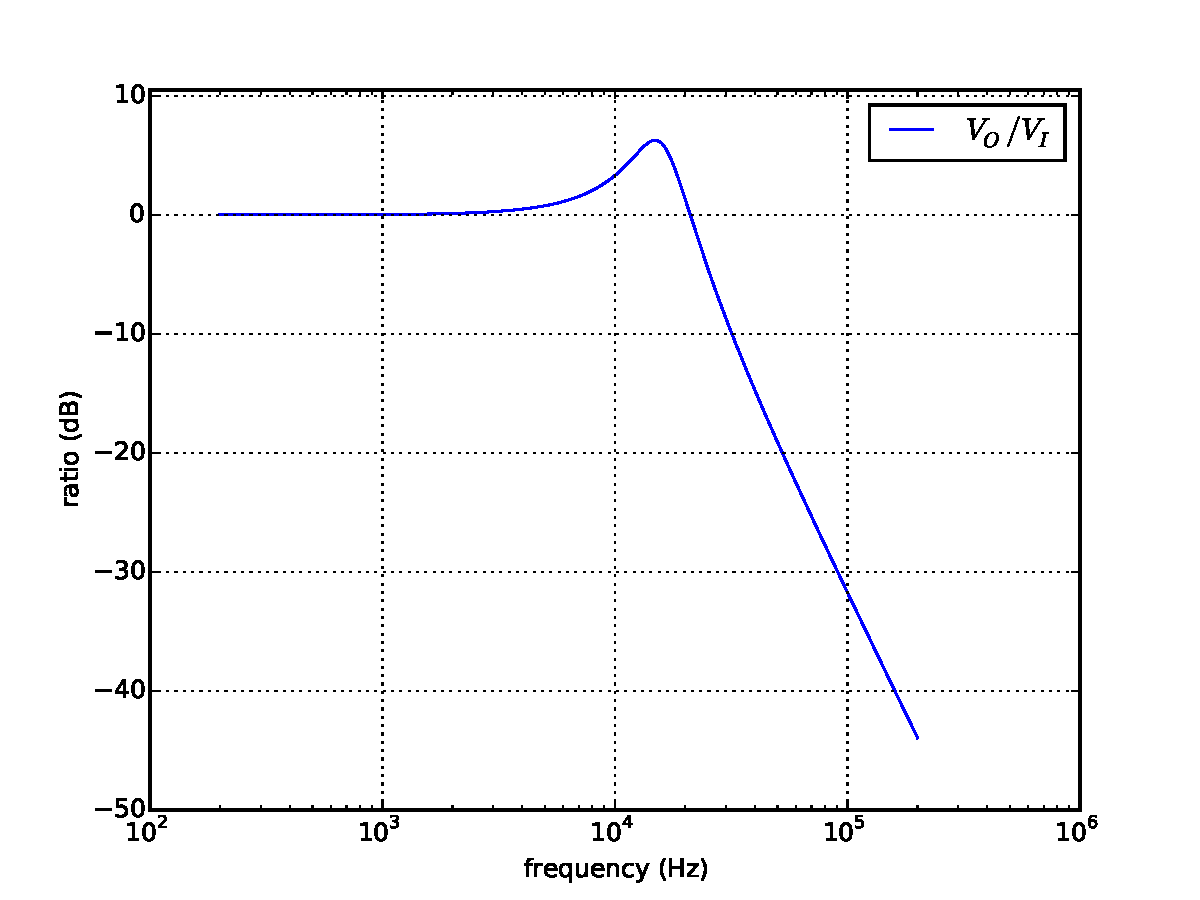
\includegraphics[width=1\textwidth]{circuit/p13.pdf}
          \caption{$\SI{2}\kohm$}
        \end{subfigure}
        \caption{電路(1)}
      \end{figure}

      \item 高通電路  \begin{figure}[H]
        \centering
        \begin{subfigure}[b]{0.45\textwidth}
          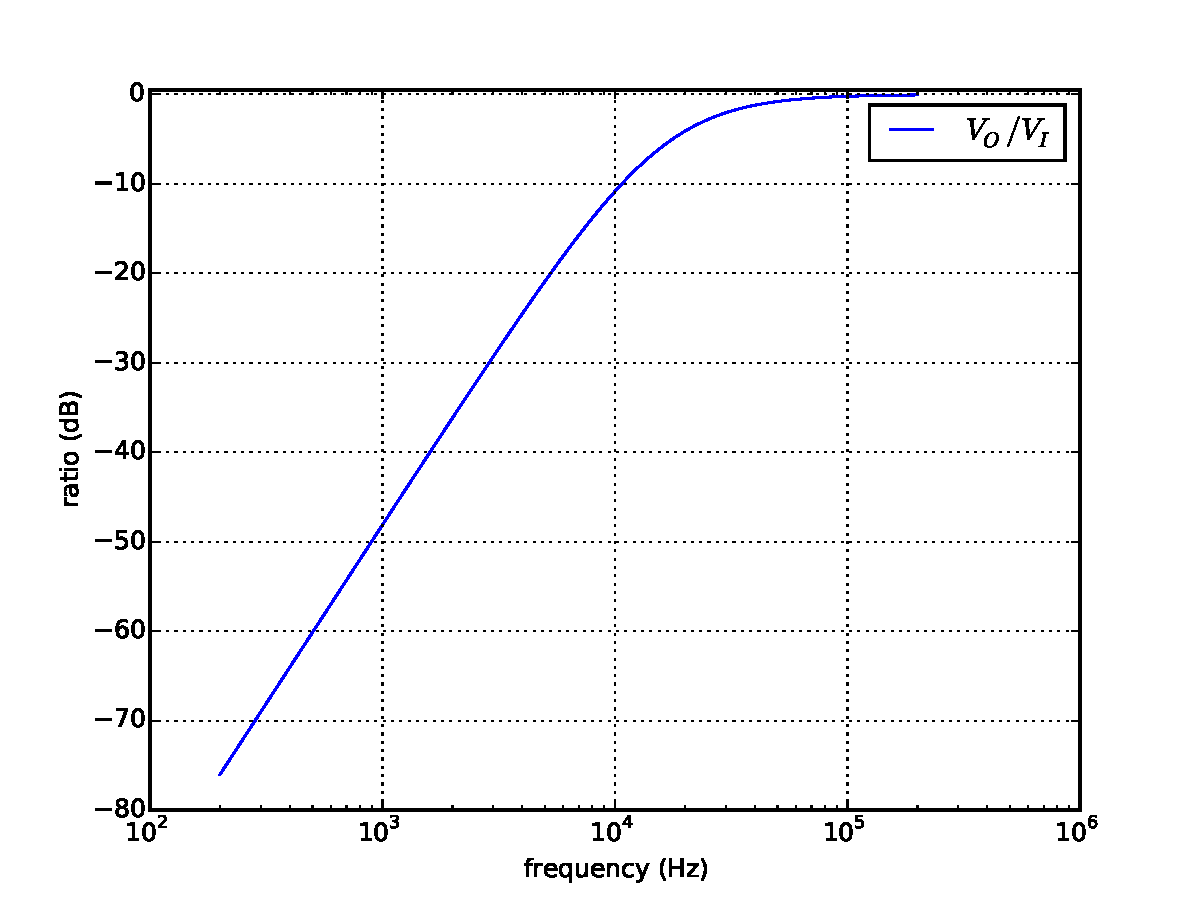
\includegraphics[width=1\textwidth]{circuit/p21.pdf}
          \caption{$\SI{510}\ohm$}
        \end{subfigure}
        \begin{subfigure}[b]{0.45\textwidth}
          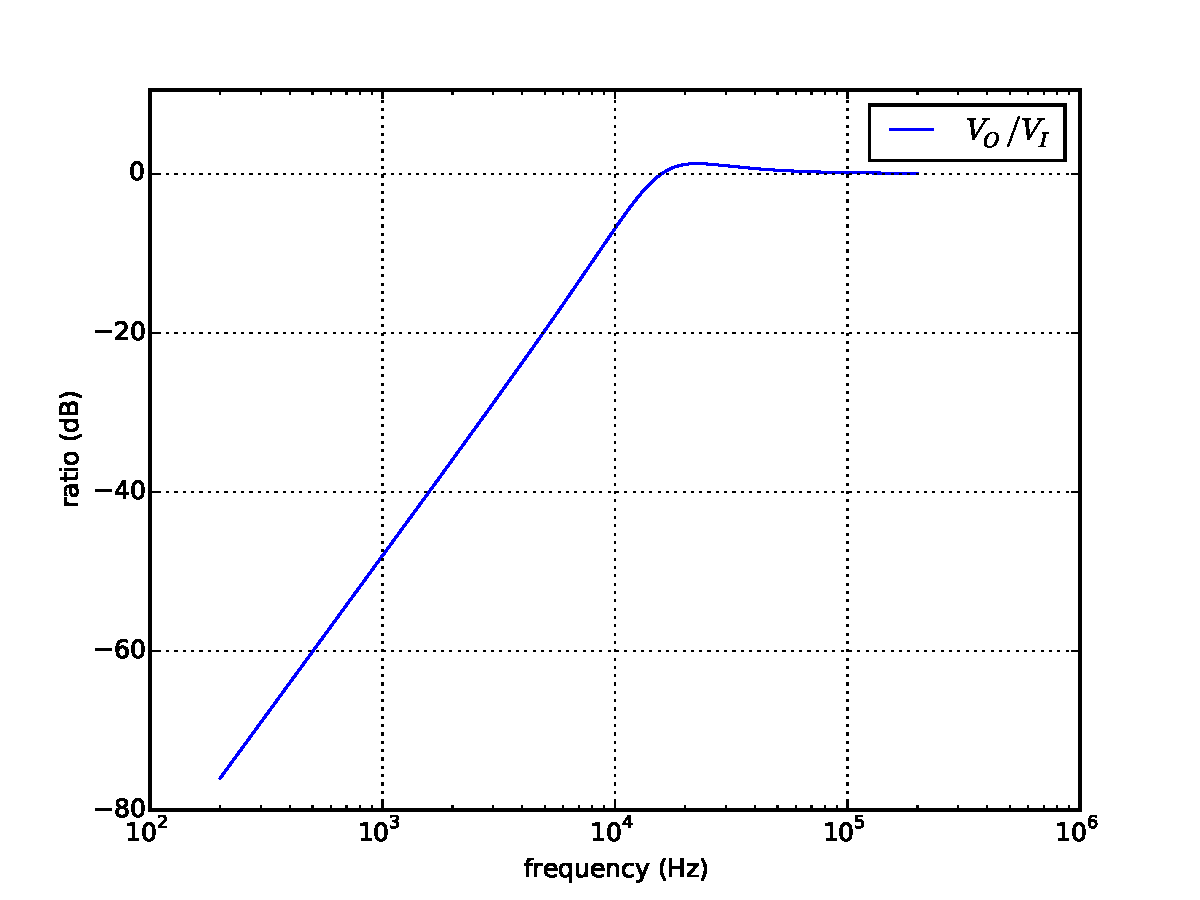
\includegraphics[width=1\textwidth]{circuit/p22.pdf}
          \caption{$\SI{1}\kohm$}
        \end{subfigure}
        \begin{subfigure}[b]{0.45\textwidth}
          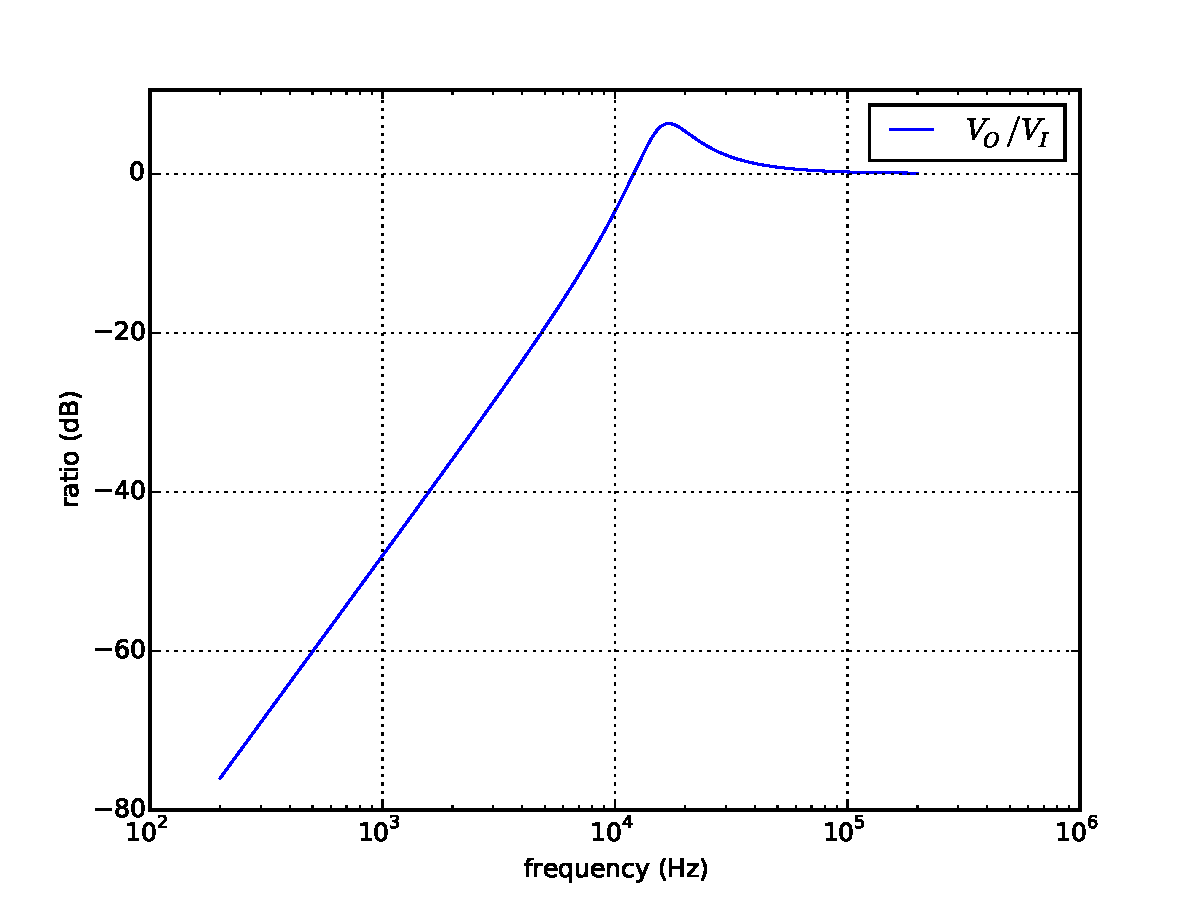
\includegraphics[width=1\textwidth]{circuit/p23.pdf}
          \caption{$\SI{2}\kohm$}
        \end{subfigure}
        \caption{電路(2)}
      \end{figure}
      \clearpage

      \item 帶通電路  \begin{figure}[H]
        \centering
        \begin{subfigure}[b]{0.45\textwidth}
          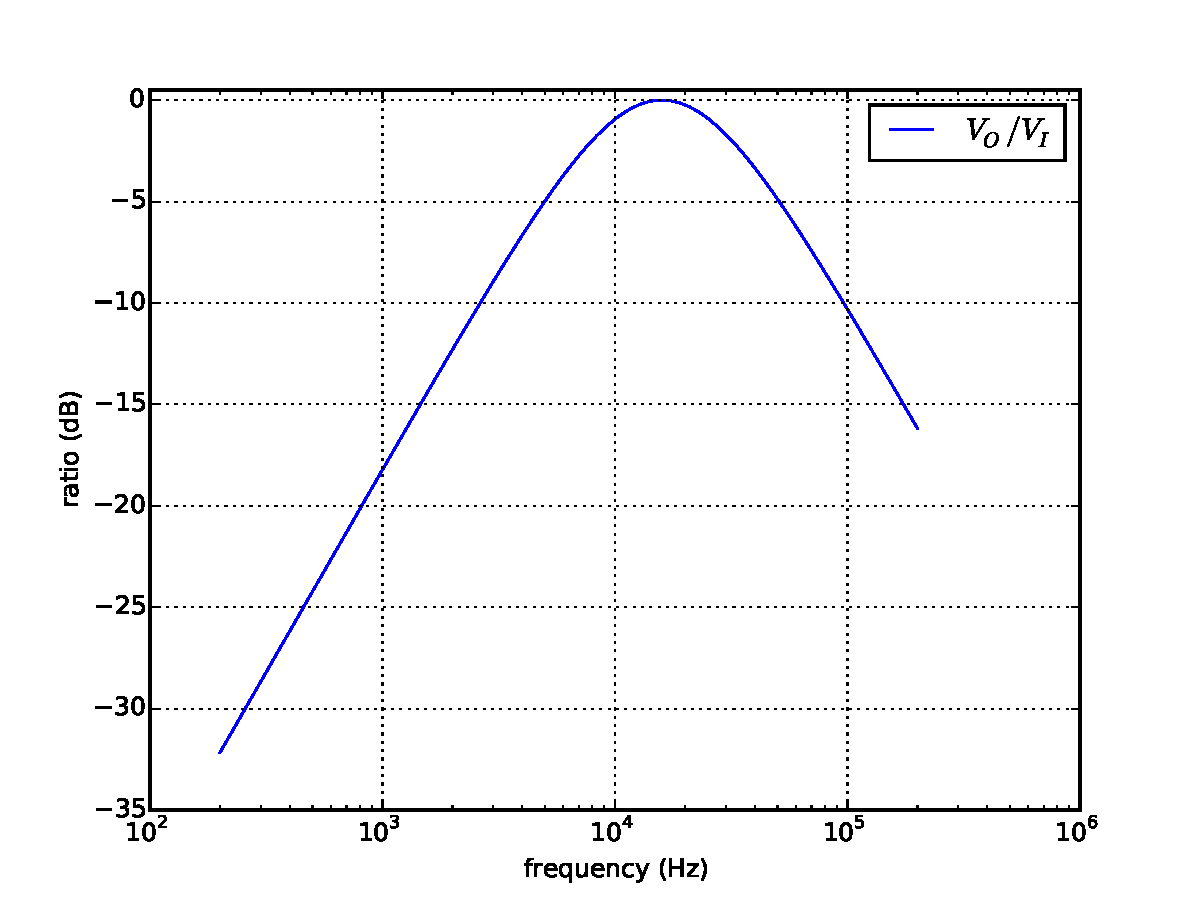
\includegraphics[width=1\textwidth]{circuit/p31.pdf}
          \caption{$\SI{510}\ohm$}
        \end{subfigure}
        \begin{subfigure}[b]{0.45\textwidth}
          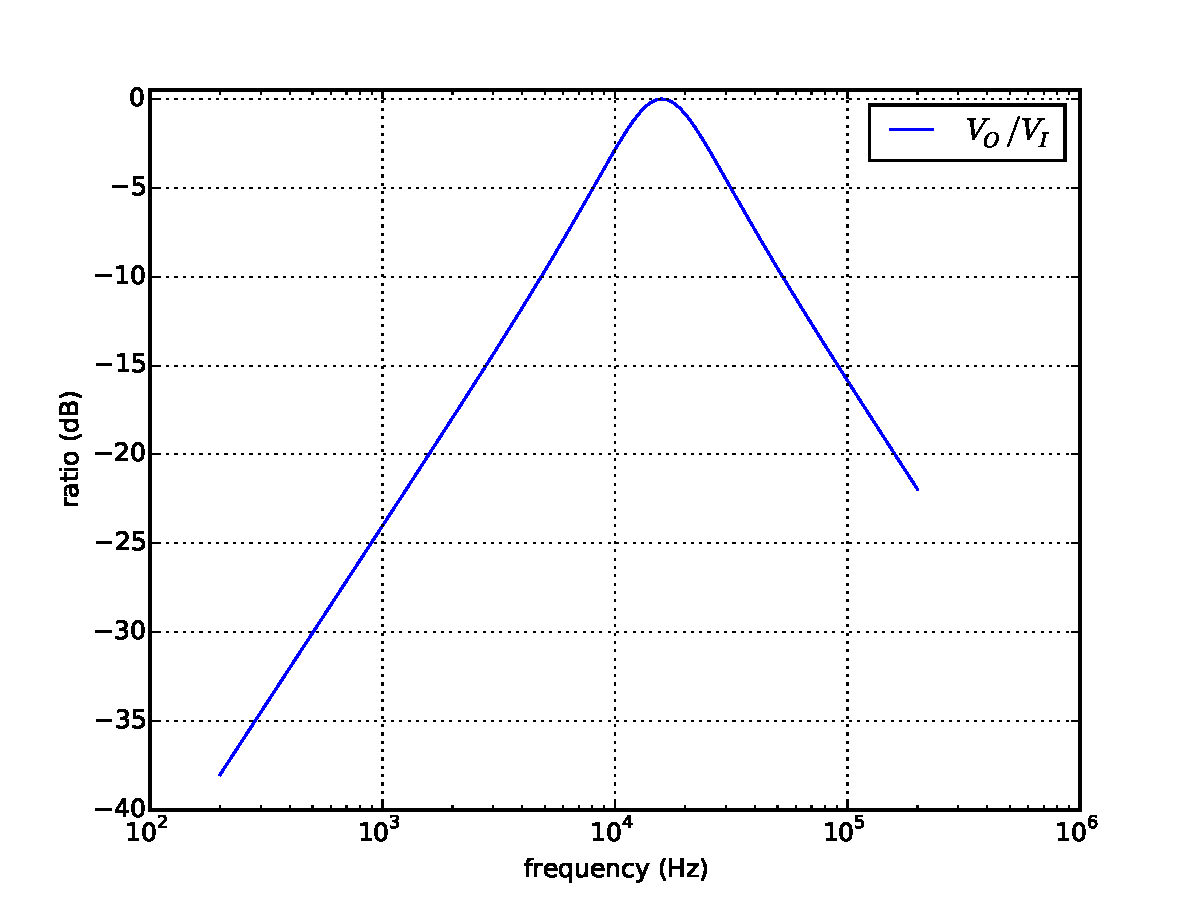
\includegraphics[width=1\textwidth]{circuit/p32.pdf}
          \caption{$\SI{1}\kohm$}
        \end{subfigure}
        \begin{subfigure}[b]{0.45\textwidth}
          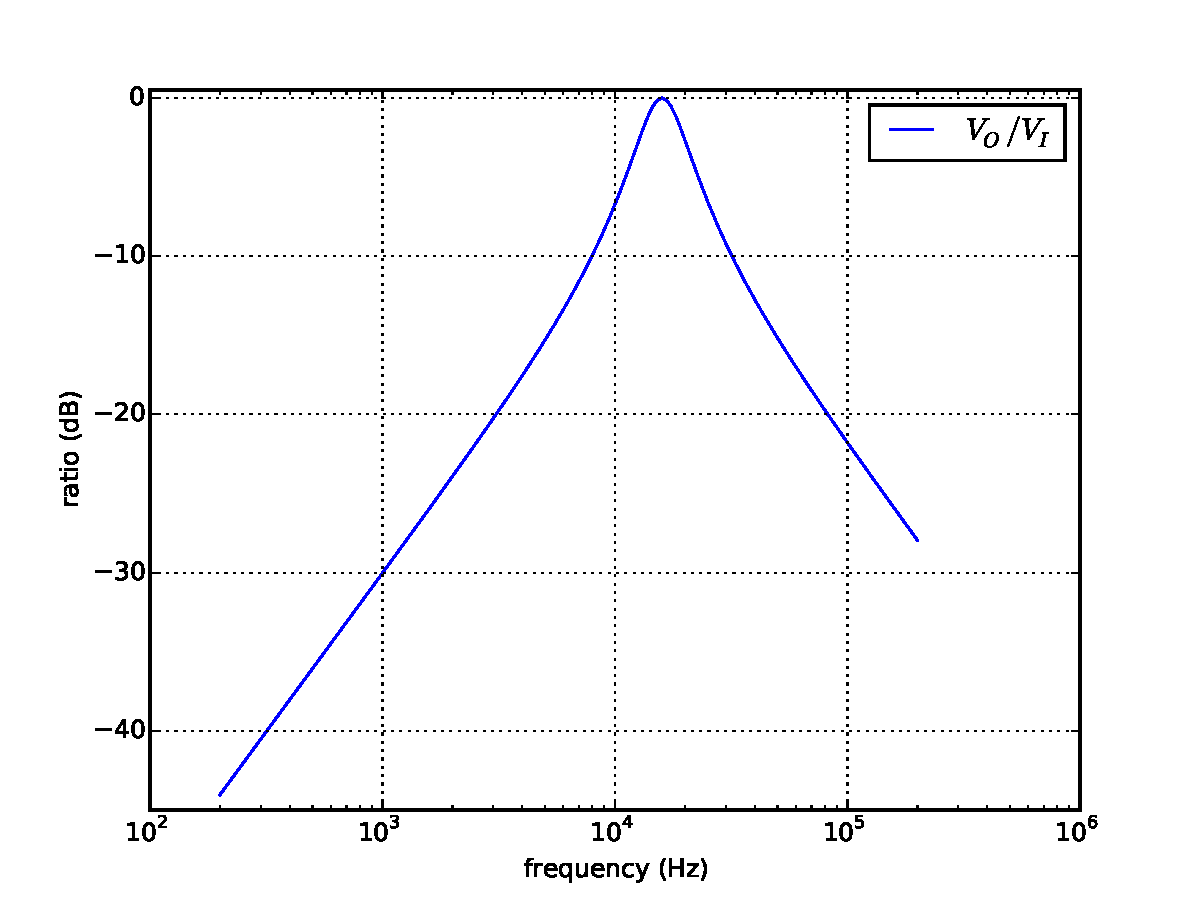
\includegraphics[width=1\textwidth]{circuit/p33.pdf}
          \caption{$\SI{2}\kohm$}
        \end{subfigure}
        \caption{電路(3)}
      \end{figure}
    \end{enumerate}

\end{enumerate}

\end{document}


